\documentclass{article}[11pt]

\usepackage{amssymb}
\usepackage{amsmath}
\usepackage{calc}
\usepackage{gensymb}
\usepackage[margin=0.5in]{geometry}
\usepackage{graphicx}
\usepackage{tikz}
\usepackage{tikz-3dplot}
\usepackage{epstopdf}
\usepackage{enumitem}
\usepackage{pgfplots}


% pdf versions
\pdfoptionpdfminorversion=7

% handle page stretching
\raggedbottom

% Use for drawings
\usetikzlibrary{angles,arrows,calc,decorations,intersections,patterns,positioning,quotes,shapes}

\tikzset{% Tikz commands for drawing block diagrams, etc...
	block/.style    = {draw, rectangle, minimum height = 2em, minimum width = 2em},
	sum/.style      = {draw, circle}, % Adder
	input/.style    = {fill=white, rectangle}, % Input
	output/.style   = {fill=white, rectangle}, % Output
	waypoint/.style   = {coordinate}, % Output
}

% Define Laplace, Fourier transform symbols
\newcommand{\LT}{\mathcal{L}}
\newcommand{\FT}{\mathcal{F}}
\newcommand{\adj}{\text{adj}}
\newcommand{\rank}{\text{rank}}
\newcommand{\jw}{j\omega}
\newcommand{\spl}{s\textrm{-plane}}
\newcommand{\wt}{\omega t}
\newcommand{\Lm}{\textrm{Lm }}
\newcommand{\logg}{\log_{10}}

% Clean up overline/underline for math mode
\def\obar#1{\bar{#1}}
\def\ubar#1{\ushort{#1}}



\begin{document}$  $\vspace{4em}
	
\noindent	
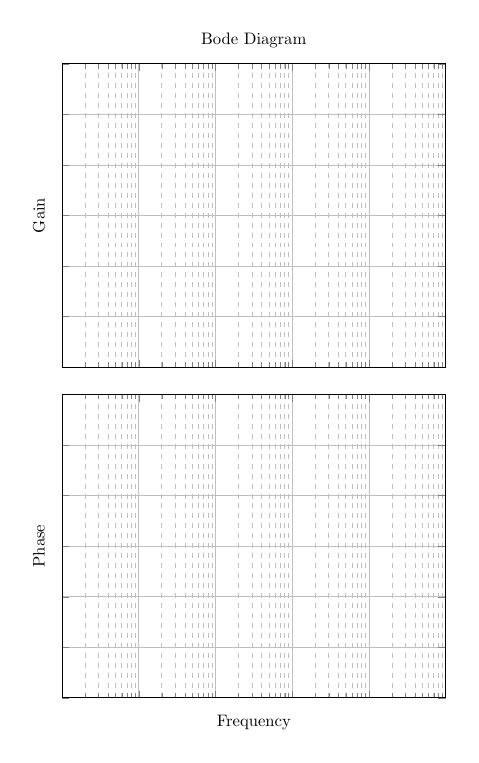
\begin{tikzpicture}[scale=0.6]
\begin{scope}[trim axis left,trim axis right]
\begin{semilogxaxis}[title=Bode Diagram, ylabel=Gain, xmin=1e-1, xmax=1e4, ymin=-60, ymax=60, yticklabels={,,}, xticklabels={,,}, width=0.8\textwidth,height=8cm,ytick={-60,-40,-20,0,20,40,60},grid=both,minor grid style={dashed}];	
\end{semilogxaxis}
\end{scope}

\begin{scope}[shift={(0,-7cm)},trim axis left,trim axis right]
\begin{semilogxaxis}[xlabel=Frequency, ylabel=Phase, xmin=1e-1, xmax=1e4, ymin=-270, ymax=0, yticklabels={,,}, xticklabels={,,}, width=0.8\textwidth,height=8cm,ytick={0,-45,-90,-135,-180,-225,-270},grid=both,minor grid style={dashed}];	
\end{semilogxaxis}
\end{scope}
\end{tikzpicture}
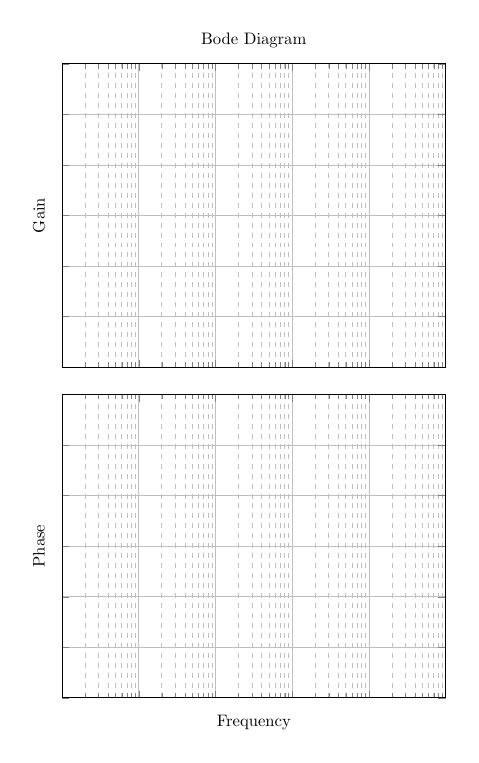
\begin{tikzpicture}[scale=0.6]
\begin{scope}[trim axis left,trim axis right]
\begin{semilogxaxis}[title=Bode Diagram, ylabel=Gain, xmin=1e-1, xmax=1e4, ymin=-60, ymax=60, yticklabels={,,}, xticklabels={,,}, width=0.8\textwidth,height=8cm,ytick={-60,-40,-20,0,20,40,60},grid=both,minor grid style={dashed}];	
\end{semilogxaxis}
\end{scope}

\begin{scope}[shift={(0,-7cm)},trim axis left,trim axis right]
\begin{semilogxaxis}[xlabel=Frequency, ylabel=Phase, xmin=1e-1, xmax=1e4, ymin=-270, ymax=0, yticklabels={,,}, xticklabels={,,}, width=0.8\textwidth,height=8cm,ytick={0,-45,-90,-135,-180,-225,-270},grid=both,minor grid style={dashed}];	
\end{semilogxaxis}
\end{scope}
\end{tikzpicture}

\vfill

\noindent
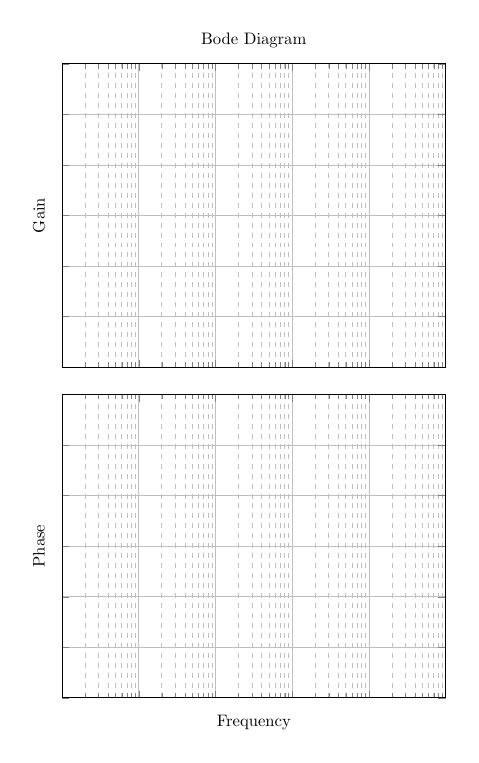
\begin{tikzpicture}[scale=0.6]
\begin{scope}[trim axis left,trim axis right]
\begin{semilogxaxis}[title=Bode Diagram, ylabel=Gain, xmin=1e-1, xmax=1e4, ymin=-60, ymax=60, yticklabels={,,}, xticklabels={,,}, width=0.8\textwidth,height=8cm,ytick={-60,-40,-20,0,20,40,60},grid=both,minor grid style={dashed}];	
\end{semilogxaxis}
\end{scope}

\begin{scope}[shift={(0,-7cm)},trim axis left,trim axis right]
\begin{semilogxaxis}[xlabel=Frequency, ylabel=Phase, xmin=1e-1, xmax=1e4, ymin=-270, ymax=0, yticklabels={,,}, xticklabels={,,}, width=0.8\textwidth,height=8cm,ytick={0,-45,-90,-135,-180,-225,-270},grid=both,minor grid style={dashed}];	
\end{semilogxaxis}
\end{scope}
\end{tikzpicture}
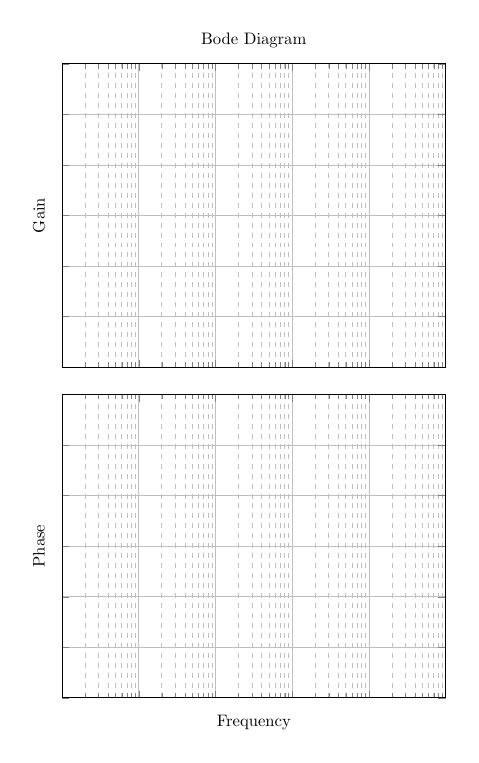
\begin{tikzpicture}[scale=0.6]
\begin{scope}[trim axis left,trim axis right]
\begin{semilogxaxis}[title=Bode Diagram, ylabel=Gain, xmin=1e-1, xmax=1e4, ymin=-60, ymax=60, yticklabels={,,}, xticklabels={,,}, width=0.8\textwidth,height=8cm,ytick={-60,-40,-20,0,20,40,60},grid=both,minor grid style={dashed}];	
\end{semilogxaxis}
\end{scope}

\begin{scope}[shift={(0,-7cm)},trim axis left,trim axis right]
\begin{semilogxaxis}[xlabel=Frequency, ylabel=Phase, xmin=1e-1, xmax=1e4, ymin=-270, ymax=0, yticklabels={,,}, xticklabels={,,}, width=0.8\textwidth,height=8cm,ytick={0,-45,-90,-135,-180,-225,-270},grid=both,minor grid style={dashed}];	
\end{semilogxaxis}
\end{scope}
\end{tikzpicture}

\vfill

\end{document}